%%%%%%%%%%%%%%%%%%%%%%%%%%%%%%%
%This is the article LaTeX template for RSC journals
%Copyright The Royal Society of Chemistry 2010
%%%%%%%%%%%%%%%%%%%%%%%%%%%%%%%

\documentclass[8.5pt,twoside,twocolumn]{article}
\oddsidemargin -1.2cm
\evensidemargin -1.2cm
\textwidth 18cm
\headheight 1.0in
\topmargin -3.5cm
\textheight 22cm
\usepackage[super,sort&compress,comma]{natbib} 
\usepackage{mhchem}
\usepackage{times,mathptmx}
% \usepackage{times}
% feel free not to use mathptmx if it causes difficulties
\usepackage{sectsty}
\usepackage{balance} 

\usepackage{graphicx} %eps figures can be used instead
\usepackage{lastpage}
\usepackage[format=plain,justification=raggedright,singlelinecheck=false,font=small,labelfont=bf,labelsep=space]{caption} 
\usepackage{fancyhdr}
\pagestyle{fancy}

\begin{document}

\thispagestyle{plain}
\fancypagestyle{plain}{
\fancyhead[L]{Communication}
\fancyhead[C]{\hspace{-1cm}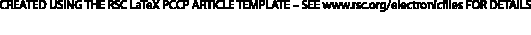
\includegraphics[height=20pt]{headers/CH}}
\fancyhead[R]{Science \vspace{-0.2cm}}
\renewcommand{\headrulewidth}{1pt}}
\renewcommand{\thefootnote}{\fnsymbol{footnote}}
\renewcommand\footnoterule{\vspace*{1pt}% 
\hrule width 3.4in height 0.4pt \vspace*{5pt}} 
\setcounter{secnumdepth}{5}



\makeatletter 
\def\subsubsection{\@startsection{subsubsection}{3}{10pt}{-1.25ex plus -1ex minus -.1ex}{0ex plus 0ex}{\normalsize\bf}} 
\def\paragraph{\@startsection{paragraph}{4}{10pt}{-1.25ex plus -1ex minus -.1ex}{0ex plus 0ex}{\normalsize\textit}} 
\renewcommand\@biblabel[1]{#1}            
\renewcommand\@makefntext[1]% 
{\noindent\makebox[0pt][r]{\@thefnmark\,}#1}
\makeatother 
\renewcommand{\figurename}{\small{Fig.}~}
\sectionfont{\large}
\subsectionfont{\normalsize} 

\fancyfoot{}
\fancyfoot[LO,RE]{\vspace{-7pt}Oregon State University 2017}
\fancyfoot[CO]{\vspace{-7.2pt}\hspace{12.2cm}Science}
\fancyfoot[RO]{\footnotesize{\sffamily{1--\pageref{LastPage} ~\textbar  \hspace{2pt}\thepage}}}
\fancyfoot[LE]{\footnotesize{\sffamily{\thepage~\textbar\hspace{3.45cm} 1--\pageref{LastPage}}}}
\fancyhead{}
\renewcommand{\headrulewidth}{1pt} 
\renewcommand{\footrulewidth}{1pt}
\setlength{\arrayrulewidth}{1pt}
\setlength{\columnsep}{6.5mm}
\setlength\bibsep{1pt}

\twocolumn[
  \begin{@twocolumnfalse}
\noindent\LARGE{\textbf{Identification of an unknown disubstituted benzene derivative}}
\vspace{0.6cm}

\noindent\large{\textbf{Elliott Capek,\textit{$^{a}$} Steven Nguyen,\textit{$^{b\ddag}$} Kristin Ziebart,\textit{$^{b\ddag}$} Kevin Gable\textit{$^{b}$}}}\vspace{0.2cm}
%Please note that \ast indicates the corresponding author(s) but no footnote text is required. 


\noindent\textit{\small{\textbf{Received 22\textit{$^{nd}$} March 2017, Accepted 27\textit{$^{th}$} March 2017}}}\newline

\vspace{0cm}
%Please do not change this text.

\noindent \normalsize{Small organic molecules give off distinct signals in mass spectrometry (MS) and NMR. MS of an unknown disubstituted benzene (codename \textit{Sample 8}) produces a spectra indicating a mass of $136$ atomic mass units (amu). $^{13}$C NMR suggests a total of 8 carbons present in the molecule, six being aromatic, one carboxylic and the other methyl. $^{1}$H-NMR and analysis of molecular mass confirm \textit{Sample 8} as a likely methyl benzoic acid. $^{1}$H-NMR splitting patterns, namely a lack of a singlet peak and presence of four unique aromatic hydrogens, suggest the \textit{meta} substitution pattern. $^{13}$C-$^{1}$H HMBC and HSQC experiments validate this designation. Thus \textit{Sample 8} is given the designation \textit{3-methylbenzoic acid}.}
\vspace{0.5cm}
 \end{@twocolumnfalse}
  ]


\section{Introduction}
%Footnotes

%Please use \dag to cite the ESI in the main text of the article.
%If you article does not have ESI please remove the the \dag symbol from the title and the above footnotetext.

\footnotetext{\textit{$^{a}$~Department of Physics, Oregon State University, Corvallis, Oregon, USA. E-mail: capeke@oregonstate.edu}}
\footnotetext{\textit{$^{b}$~Department of Chemistry, Oregon State University, Corvallis, Oregon, USA}}
\footnotetext{\textit{\ddag~ Authors contributed equally to this work.}}

%additional addresses can be cited as above using the lower-case letters, c, d, e... If all authors are from the same address, no letter is required

Mass spectrometry (MS) and NMR are invaluable techniques for structure elucidation of unknown organic molecules. When a molecule is sufficiently simple, knowledge of its molecular weight, carbon number, and the shifts of its carbons and hydrogens can be enough to uniquely determine identity. For more complex molecules, or those with many isomers, further information from 2D experiments like $^{13}$C-$^{1}$H HSQC or $^{13}$C-$^{1}$H HMBC may be necessary.\\

This article follows the designation of a disubstituted benzene unknown using the above techniques. MS is used to determine weight, $^{13}$C NMR is used to come up with a candidate structure, $^{1}$H NMR is used to verify this candidate and guess its substitution, and $^{13}$C-$^{1}$H HSQC/HMBC are used to verify the substitution.\\

\section{MS}
Molecular mass is first determined by examining the MS spectra shown in Figure \ref{fig:MS}. The largest peak in the highest M/Z ratio peak group is at 136 M/Z, indicating the molecular weight of the unknown is 135 g/mol.\\

The intensity ratio of the major 136 peak and the 137 peak is 0.89, which matches with the theoretical ratio of $0.011*8 = 0.88$ for an 8-carbon molecule.\\

\begin{figure}[h]
\centering
  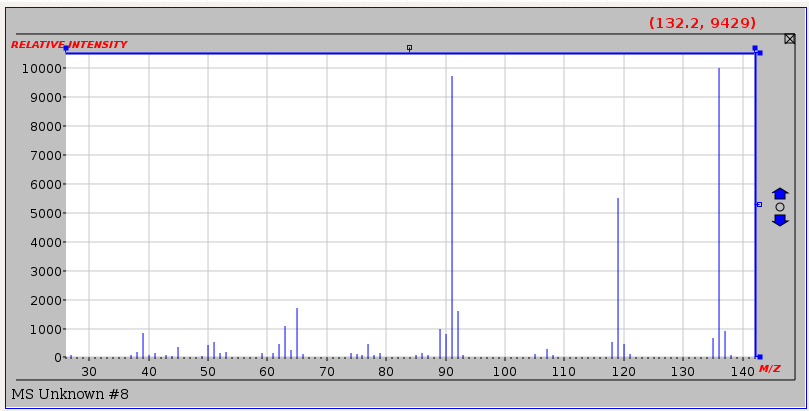
\includegraphics[height=5cm]{figures/MS.png}
  \caption{Mass spectrometry spectra of \textit{Sample 8}.}
  \label{fig:MS}
\end{figure}

\section{$^{13}$C NMR}
The $^{13}$C NMR spectra shown in Figure \ref{fig:CNMR} has 9 peaks. Comparison with online shift reports [2] indicate one peak is due to a DMSO solvent, six to aromatic carbons, one to a methyl carbon and one to a carboxylic carbon, as shown in Table \ref{table:MS}. These results agree with the 8-carbon estimate from peak ratios in MS.\\

\begin{figure}[h]
\centering
  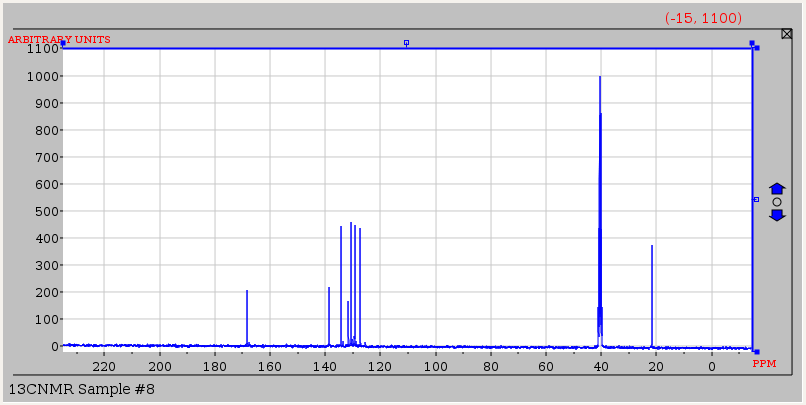
\includegraphics[height=4.5cm]{figures/CNMR.png}
  \caption{$^{13}$C NMR of \textit{Sample 8}.}
  \label{fig:CNMR}
\end{figure}

\begin{table}[h]
\small
  \caption{$^{13}$C NMR identified peaks for spectra shown in Figure \ref{fig:CNMR}.}
  \label{table:MS}
  \begin{tabular*}{0.5\textwidth}{@{\extracolsep{\fill}}lll}
    \hline
    Peak(s) shift(s) ppm & Designation \\
    \hline
    22 & Methyl carbon \\
    40 & DMSO solvent\\
    130-140 & 6x Aromatic carbons\\
    168 & Carboxylic carbon\\
    \hline
  \end{tabular*}
\end{table}

\section{$^{1}$H NMR}
$^{1}$H NMR is then used to get more information on substitutuent placement. A spectra is shown in Figure \ref{fig:HNMR} with annotated peaks shown in Table \ref{table:HNMR} indicating the presence of a carboxylic hydrogen at 12.8ppm and methyl hydrogens at 2.3ppm [2], verifying the methyl benzoic acid hypothesis. The splitting pattern of the aromatic hydrogens shown in Figure \ref{fig:HNMR-closeup} is used to determine configuration. Because four unique aromatic peaks are visible, the \textit{para} configuration is impossible. The presence of a singlet aromatic peak rules out \textit{ortho} and suggests \textit{meta} as the substitution pattern.\\

The \textit{meta} designation is further evidenced by the presence of very small, 1-Hz meta coupling of the two doublet hydrogens. This coupling is expected between the singlet hydrogen and the two hydrogens adjacent to only one substitute group.\\

\begin{figure}[h]
\centering
  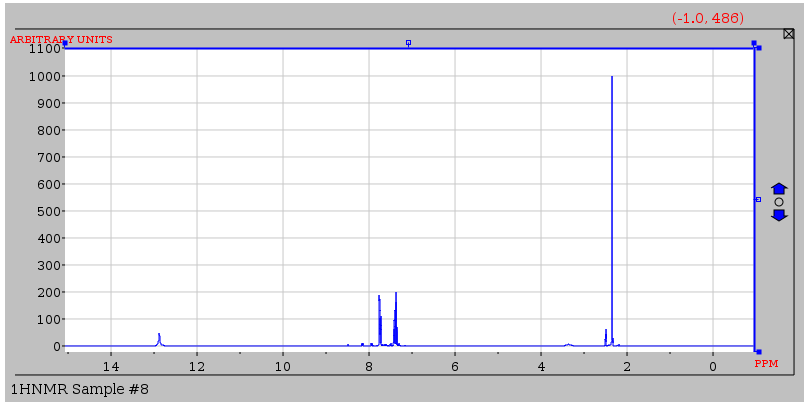
\includegraphics[height=4cm]{figures/HNMR.png}
  \caption{$^{1}$H NMR of \textit{Sample 8}.}
  \label{fig:HNMR}
\end{figure}

\begin{figure}[h]
\centering
  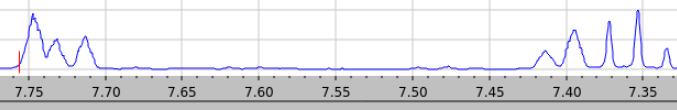
\includegraphics[height=1.2cm]{figures/HNMR-splitting.png}
  \caption{Close-up of aromatic peaks in $^{1}$H NMR spectra of \textit{Sample 8}.}
  \label{fig:HNMR-closeup}
\end{figure}

\begin{table}[h]
\small
  \caption{$^{1}$H NMR identified peaks for spectra shown in Figure \ref{fig:HNMR}.}
  \label{table:HNMR}
  \begin{tabular*}{0.5\textwidth}{@{\extracolsep{\fill}}llll}
    \hline
    Shift(s) ppm & Integration & Splitting & Designation \\
    \hline
    2.3 & 3.1 & Singlet & Ar-CH$_3$ hydrogens\\
    2.4 & 0.4 & Pentet & DMSO\\
    7.35 & 1.1 & Singlet & Aromatic H\\
    7.4 & 1.0 &  Meta Doublet & Aromatic H\\
    7.72 & 1.1 & Meta Doublet & Aromatic H\\
    7.75 & 1.1 & Singlet & Aromatic H\\
    12.8 & 1.0 & Singlet & Carboxylic H\\
    \hline
  \end{tabular*}
\end{table}

\section{COSY}
The COSY spectrum of \textit{Sample 8} is not terribly useful. It verifies that aromatic hydrogens couple to one another, but HMBC provides much more information.

\begin{figure}[h]
\centering
  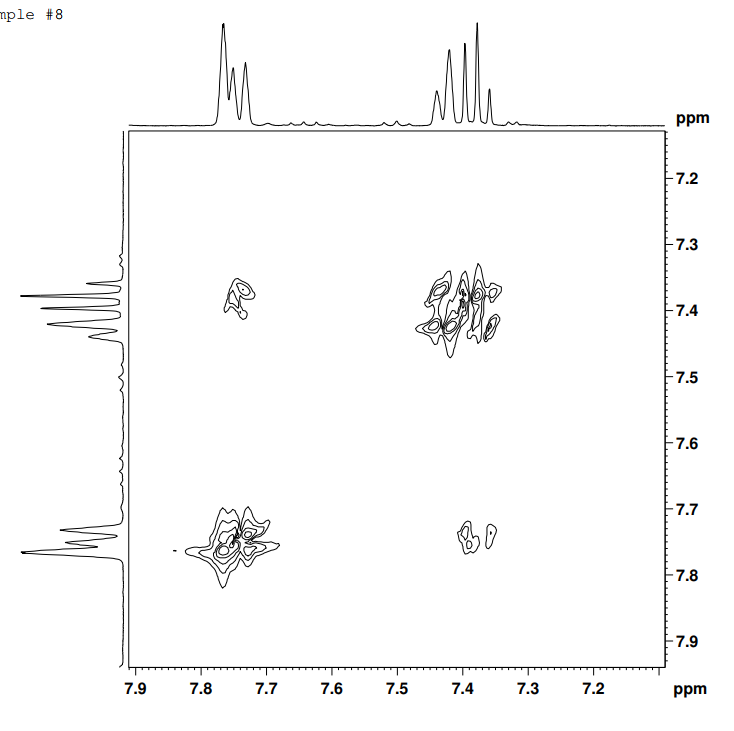
\includegraphics[height=7cm]{figures/cosy.png}
  \caption{COSY spectrum of \textit{Sample 8}.}
  \label{fig:COSY}
\end{figure}

\section{HSQC}
HSQC is similarly barren of information. The spectrum shown in Figure \ref{fig:HSQC} shows expected coupling between the solvent carbon and hydrogen, between the methyl carbon and methyl protons, and between aromatic carbons and aromatic hydrogens, as expected. More conclusively demonstrated is the presence of four different aromatic hydrogens, further verifying the molecule is not in the para configuration.\\

\begin{figure}[h]
\centering
  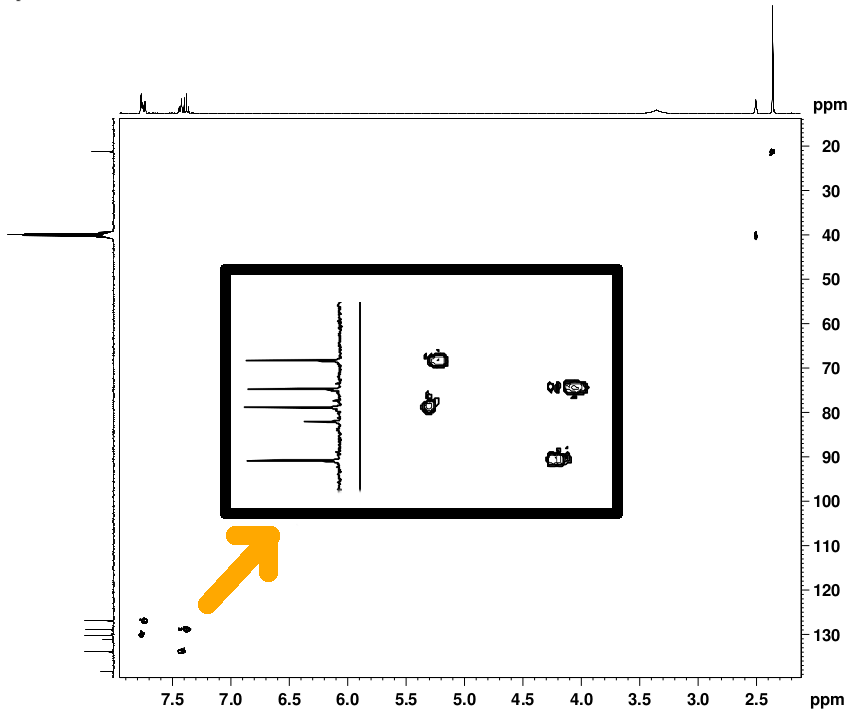
\includegraphics[height=7cm]{figures/HSQC.png}
  \caption{HSQC spectrum of \textit{Sample 8}. A blowup of the aromatic region is shown in the middle of the spectrum.}
  \label{fig:HSQC}
\end{figure}

\section{HMBC}
Now that the structure has been determined, individual carbons and hydrogens can be aligned with their respective peaks. Figure \ref{fig:3MBA} shows the candidate molecule along with labels for carbons and hydrogens.\\

\begin{figure}[h]
\centering
  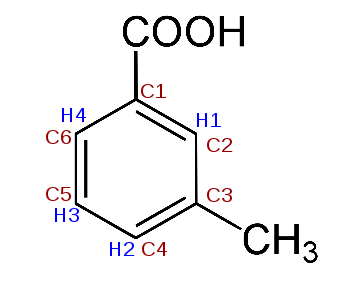
\includegraphics[height=5cm]{figures/molecule.png}
  \caption{3-methylbenzoic acid.}
  \label{fig:3MBA}
\end{figure}

Hydrogen peak placement is easy. The singlet hydrogen must correspond to the carbon between the two substituents. The triplet hydrogen must correspond to the hydrogen diametrically opposed to this carbon. This leaves the two doublet carbons. They can be distinguished by looking at the HMBC spectra shown in Figure \ref{fig:hydromethyl}. Hydrogen H2, indicated in Table \ref{table:H-peaks}, or the upfield doublet, correlates well with the methyl carbon. Carbon H4 is identified by exclusion.\\

An HMBC-HSQC overlay in the aromatic region provides much information about aromatic carbon peaks. Such a spectrum is shown in Figure \ref{fig:overlay}. Carbons C2, C4, C5 and C6 can be easily determined as the carbons which HSQC-correlate with the respective hydrogens H1, H2, H3 and H4, as shown in Table \ref{table:C-peaks}. This leaves the two substituent aromatic carbons to label. Figure \ref{fig:methylaromatic} indicates three carbons pair strongly with the methyl hydrogen: carbons C2 and C4, already labeled, and one of the two substituent carbons shifted furthest downfield of the aromatic carbons. This is likely carbon C1, since 4-bond coupling is much stronger in HMBC spectra than 2-bond coupling. Thus C1 must be the carboxylic substituent aromatic carbon, and thus C3 must be the methyl aromatic carbon. These findings are catalogued in the tables below.\\

\begin{figure}[h]
\centering
  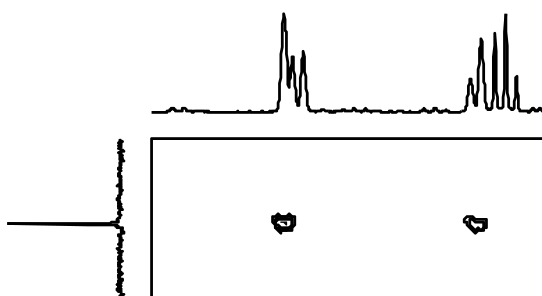
\includegraphics[height=5cm]{figures/HMBC-hydromethyl.png}
  \caption{A closeup of methyl carbon-aromatic hydrogen HMBC coupling.}
  \label{fig:hydromethyl}
\end{figure}

\begin{figure}[h]
\centering
  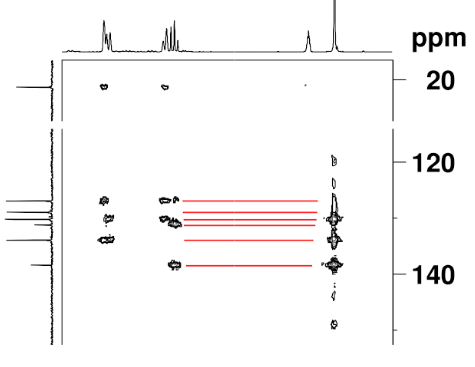
\includegraphics[height=5cm]{figures/hmbc-methylaromatic.png}
  \caption{A closeup, edited image hilighting HMBC coupling between aromatic carbons and methyl hydrogens.}
  \label{fig:methylaromatic}
\end{figure}

\begin{figure*}
\centering
  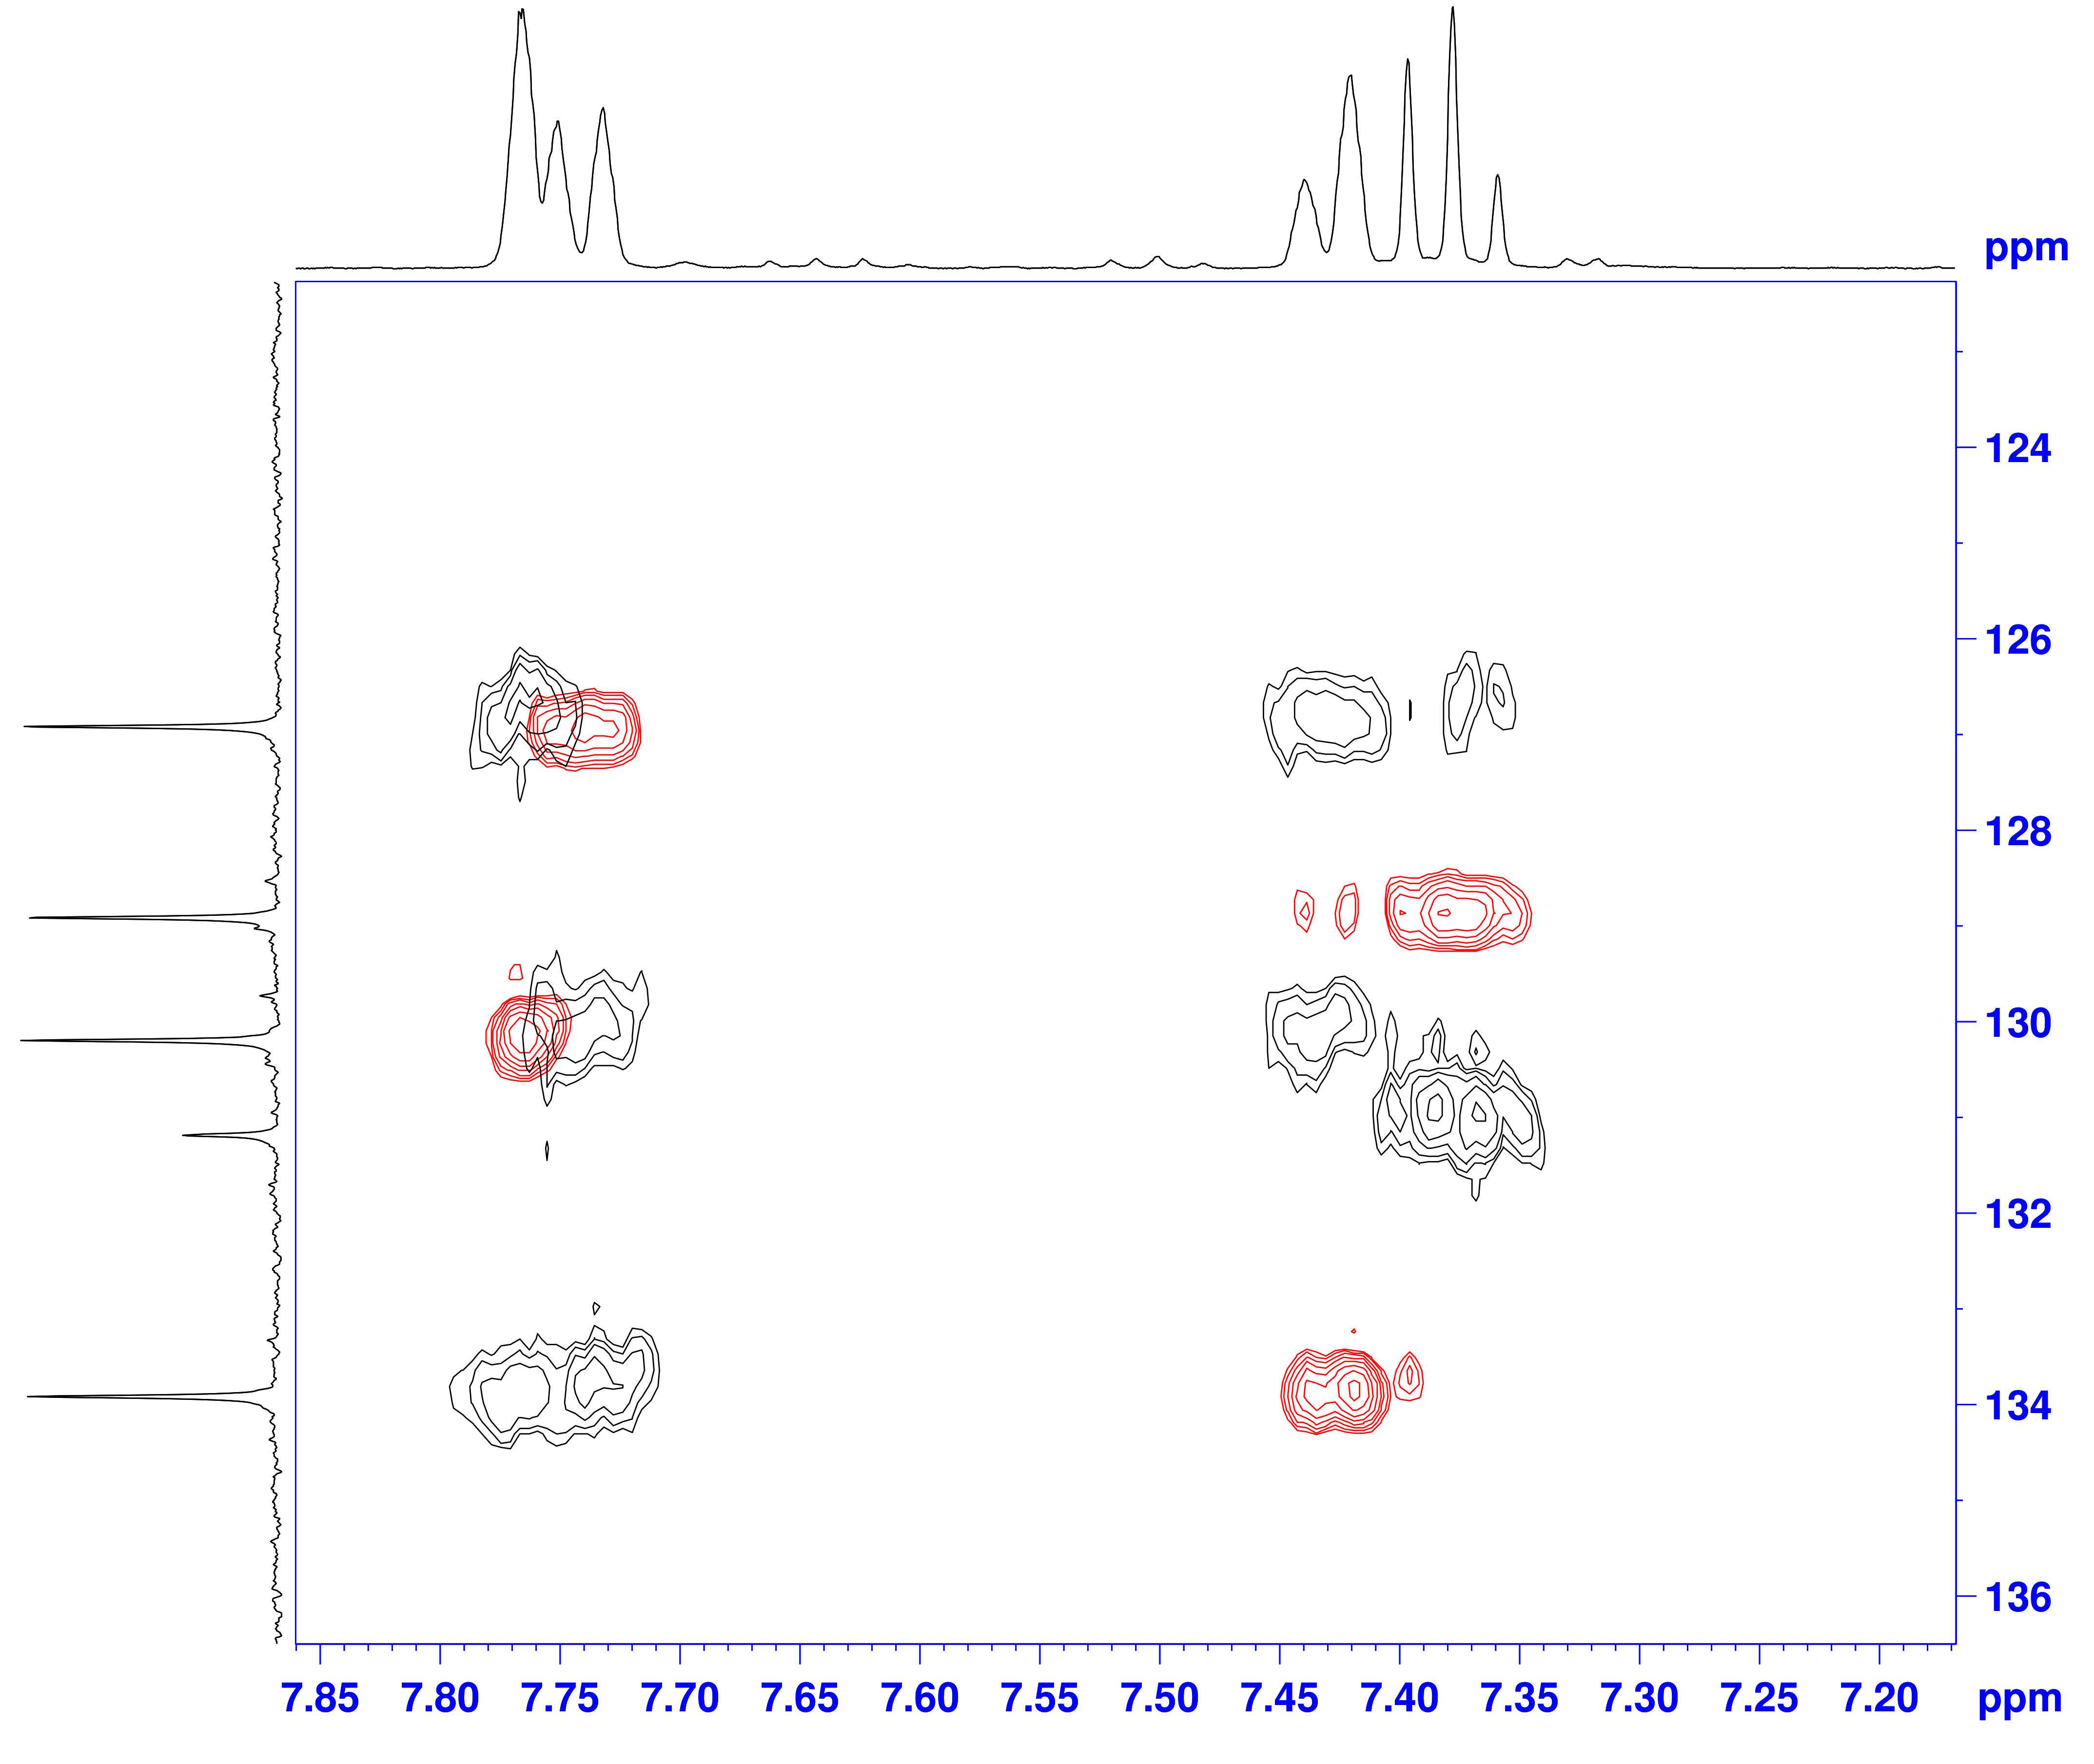
\includegraphics[height=10cm]{figures/Overlay.png}
  \caption{HSQC-HMBC overlay in the C, H aromatic region.}
  \label{fig:overlay}
\end{figure*}

\begin{table}[h]
\small
  \caption{Aromatic hydrogen peak identification. In correspondence with the labels shown in Figure \ref{fig:3MBA}.}
  \label{table:H-peaks}
  \begin{tabular*}{0.5\textwidth}{@{\extracolsep{\fill}}llll}
    \hline
    Shift(s) ppm & Designation \\
    \hline
    7.35 & H3 triplet hydrogen\\
    7.4  & H2 doublet hydrogen\\
    7.72 & H4 doublet hydrogen\\
    7.75 & H1 singlet hydrogen\\
    \hline
  \end{tabular*}
\end{table}

\begin{table}[h]
\small
  \caption{Aromatic carbon peak identification. In correspondence with the labels shown in Figure \ref{fig:3MBA}.}
  \label{table:C-peaks}
  \begin{tabular*}{0.5\textwidth}{@{\extracolsep{\fill}}llll}
    \hline
    Shift(s) ppm & Designation \\
    \hline
    127 & Carbon 6\\
    129 & Carbon 5\\
    130 & Carbon 2\\
    131 & Carbon 3\\
    134 & Carbon 4\\
    139 & Carbon 1\\
    \hline
  \end{tabular*}
\end{table}

% an example of a two-column figure
%% \begin{figure*}
%%   \centering
%%   \includegraphics[height=3cm]{example.jpg}
%%   \caption{An example figure caption, an image from the \textit{Physical Chemistry Chemical Physics} cover gallery.}
%%   \label{fgr:example}
%% \end{figure*}

% an example of a two-column table
%\begin{table*}
%\small
  %\caption{\ An example of a caption to accompany a table, table captions do not end in a full point}
  %\label{tbl:example}
  %\begin{tabular*}{\textwidth}{@{\extracolsep{\fill}}lllllll}
    %\hline
    %Header one & Header two & Header three & Header four & Header five & Header six  & Header seven\\
    %\hline
    %1 & 2 & 3 & 4 & 5 & 6  & 7\\
    %8 & 9 & 10 & 11 & 12 & 13 & 14 \\
    %15 & 16 & 17 & 18 & 19 & 20 & 21\\
    %\hline
  %\end{tabular*}
%\end{table*}


%The \balance command can be used to balance the columns on the final page if desired. It should be placed anywhere within the first column of the last page.

%\balance

%If notes are included in your references you can change the title from 'References' to 'Notes and references' using the following command:
%\renewcommand\refname{Notes and references}

\begin{@twocolumnfalse}
\section{References}
[1] Experimental Chemistry I: CH 362, OSU Department of Chemistry 2017\\

[2] OSU of Chemistry. 1H NMR Chemical Shifts. http://www.science.oregonstate.edu/~gablek/CH335/Chapter10/ChemicalShift.htm. (Accessed March 22, 2017)\\
\end{@twocolumnfalse}
\end{document}
